% !TEX TS-program = pdflatex
% !TEX encoding = UTF-8 Unicode

% This is a simple template for a LaTeX document using the "article" class.
% See "book", "report", "letter" for other types of document.

\documentclass[11pt]{article} % use larger type; default would be 10pt

\usepackage[utf8]{inputenc} % set input encoding (not needed with XeLaTeX)

%%% Examples of Article customizations
% These packages are optional, depending whether you want the features they provide.
% See the LaTeX Companion or other references for full information.

%%% PAGE DIMENSIONS
\usepackage{geometry} % to change the page dimensions
\geometry{a4paper} % or letterpaper (US) or a5paper or....
\geometry{margin=1in} % for example, change the margins to 2 inches all round
% \geometry{landscape} % set up the page for landscape
%   read geometry.pdf for detailed page layout information

\usepackage{graphicx} % support the \includegraphics command and options

% \usepackage[parfill]{parskip} % Activate to begin paragraphs with an empty line rather than an indent

%%% PACKAGES
\usepackage{booktabs} % for much better looking tables
\usepackage{array} % for better arrays (eg matrices) in maths
\usepackage{paralist} % very flexible & customisable lists (eg. enumerate/itemize, etc.)
\usepackage{verbatim} % adds environment for commenting out blocks of text & for better verbatim
\usepackage{subfig} % make it possible to include more than one captioned figure/table in a single float
% These packages are all incorporated in the memoir class to one degree or another...
\usepackage{amsmath}
\usepackage{amssymb}
\usepackage{graphicx}
\usepackage{float}
\usepackage{multirow}
%%% HEADERS & FOOTERS
\usepackage{fancyhdr} % This should be set AFTER setting up the page geometry
\pagestyle{fancy} % options: empty , plain , fancy
\renewcommand{\headrulewidth}{0pt} % customise the layout...
\lhead{}\chead{}\rhead{}
\lfoot{}\cfoot{\thepage}\rfoot{}

\usepackage[
singlelinecheck=false % <-- important
]{caption}


%%% SECTION TITLE APPEARANCE
\usepackage{sectsty}
\allsectionsfont{\sffamily\mdseries\upshape} % (See the fntguide.pdf for font help)
% (This matches ConTeXt defaults)

%%% ToC (table of contents) APPEARANCE
\usepackage[nottoc,notlof,notlot]{tocbibind} % Put the bibliography in the ToC
\usepackage[titles,subfigure]{tocloft} % Alter the style of the Table of Contents
\renewcommand{\cftsecfont}{\rmfamily\mdseries\upshape}
\renewcommand{\cftsecpagefont}{\rmfamily\mdseries\upshape} % No bold!


\begin{document}
\title{Missing Value Imputation using Low Rank Models}


\maketitle
\noindent
In this analysis we compare the standard imputation algorithm in Social Sciences, Multiple Imputation with imputations obtained via Low Rank matrix completion algorithms, including trace norm regularization. 
\section{Imputation Techniques}
Given an observed dataset $df_{obs}$, with $N_{obs}$ entries, we apply the following $5$ imputation techniques to obtain imputed values of the missing datapoints $N_{miss}$:
\begin{itemize}
\item[1] GLRM (Generalized Low Rank Models) on scaled data -- where the low rank `k' is picked via $5-$fold crossvalidation.   
\item[2] GLRM on unscaled data --  where the low rank `k' is picked via $5-$fold crossvalidation.   
\item[3] Trace Norm regularization on the Full Rank model -- where the regularization constant $\alpha$ is picked via $5$-fold crossvalidation, and the rank of the model is kept fixed at the full rank. 
\item[4] Trace Norm regularization on the Low Rank model --where the regularization constant $\alpha$ is picked via $5$-fold crossvalidation, and the rank of the model is kept fixed at the low rank from the unscaled GLRM. 
\item[5] MICE (Multiple Imputation via Chained Equations) -- this is a popular implementation of the Multiple Imputation method. The algorithm involves iteratively fitting univariate regressions one column at a time using a subset of the remaining columns of the data. 
\end{itemize} 

\section{Dataset 1: General Social Survey}
The first dataset we apply the techniques to is a subsample of the General Social Survey (GSS) 2014 dataset. The GSS is a sociological survey which collects data on attitudes and demographic characteristics of adults from randomly selected households in the United States. As a first-pass we extracted a subsample of the data by:
\begin{itemize}
\item[--] removing columns corresponding to identifying variables (eg: sampling related, interviewer characteristics, interview description);
\item[--] removing columns with non-varying entries;
\item[--] removing columns with more than $33 \%$ missing entries;
\item[--] keeping only one column from pairs of very highly correlated columns (correlation$>0.70$).
\end{itemize}
The final dataset used in the analysis has $122$ columns and $2538$ rows. 

\section{Dataset 2: Simulation}
We also apply the technique to a simulated dataset.
\begin{itemize}
\item[--] Started with $25$ independent columns of length $1000$-- mix of positive real-valued, integer and boolean.
\item[--] Introduced columnwise dependencies by multiplying with a $25 \times 25$ matrix of random parameters.  
\item[--] Introduced rowwise structure by adding a random error term to each datapoint whose variance depended on the row (increasing variance with row number). 
\end{itemize}
The final dataset consists of $1000$ rows and $25$ columns ($5$ each of the types: large and positive real-valued, moderate and positive real valued, integer, boolean and categorical). 

\section{Evaluation Scheme}
The following procedure is used to compare the different imputation techniques:
\begin{itemize}
\item[1] Of the observed datapoints $N_{obs}$, $10\%$ are randomly assumed missing, these are refered to as `induced missing', labeled $N_{miss, ind}$. Let's call the resulting dataset $df_{miss, ind}$. The true value of a data point is given by $y_0$ and the imputed value is given by $\widehat{y}$.
\item[2] The 5 imputation techniques --  Low Rank (Scaled), Low Rank (Unscaled), Trace Norm (Full Rank), Trace Norm (Low Rank) and MICE are applied to $df_{miss, ind}$.
\item[3] From the resulting imputed datasets, a `loss' is calculated over the $N_{miss,ind}$ observations by comparing imputations $\widehat{y}$ to the true values $y_0$. 
\item[4] To do this, we scale all the (non-categorical) columns to ensure that each column has equal weight in the overall loss function. For all non-categorical columns we calculate quadratic loss, $Loss = (\widehat{y} - y_0)^2$, whereas for all categorical columns we calculate zero-one loss, $Loss = I (\widehat{y} \neq y_0)$. 
\end{itemize}

\section{Overall Results and Areas for Improvement}
Overall for the two datasets we consider, the GLRM techniques (particularly the Trace Norm) outperform a single imputation using MICE -- (at best about 30\% lower total loss). The main cause for concern is that while for most columns (about $80 \%$) GLRM techniques lead to $30-70 \%$ reduction in losses, for a handful of columns  (< $10 \%$) they lead to significantly \textit{higher} losses $(500-2000\%)$. \\\\
Other points to explore further include 
\begin{itemize}
\item[--] Applying the techniques to larger subsets of the GSS data as well as other social science datasets like National Longitudnal Survey of Youth.
\item[--] Working with a more advanced version of the MICE command. 
\item[--] Improving the loss metric that is used for comparisons. 
\item[--] Understanding why all five techniques still produce a handful of NA values for one or two columns.  
\item[--] Think about possibly extending GLRM to a multiple imputation setting?
\end{itemize}

\newpage

\section*{Detailed Results - GSS Subsample}
For the GSS Subsample the broad results are:
\begin{itemize}
\item[1] Overall the Trace (Full Rank) had the lowest loss, about 30\% less than a single imputation using MICE. All the LowRankModels techniques did outperform MICE in terms of the total loss.
\item[2] If we look at the column-wise losses -- in general LowRankModels had lower total column loss for most columns (88\% for Trace (Full Rank)) and most of these columns had 30-50\% lower loss than MICE.
\item[3] However for a few columns MICE had \textit{much} lower losses -- for one column it did 2000\% better. This may be an area of concern.
\item[4] If we look at the type of column, we note that Trace (Full Rank) frequently has the lowest loss values for non-categorical columns and Low Rank (Unscaled) for categorical columns.
\end{itemize}

% latex table generated in R 3.2.1 by xtable 1.7-4 package
% Wed Sep  9 16:27:42 2015
\begin{table}[H]
\caption*{Comparison of Imputation Techniques (scaled GSS data)}
\centering
\begin{tabular}{|c|c|c|c|c|c|}
  \hline
 & LowRank (S) & LowRank (NS) & Trace (FR) & Trace (LR) & MICE \\ 
  \hline
Scaled Loss/($10^3$) & 18.50 & 15.80 & 14.40 & 15.80 & 20.60 \\ 
  \%age reduction wrt MICE & 10.10 \% & 23.40 \% & 30.10  \%& 23.00 \% & -- \\ 
  \%age cols w/ lower loss & 73.50 \% & 84.60  \%& 87.20 \% & 84.60 \% & -- \\ 
   \hline
\end{tabular}
\end{table}



\begin{figure}[H]
\caption*{Percent reduction in loss on using LowRankModels vs MICE}
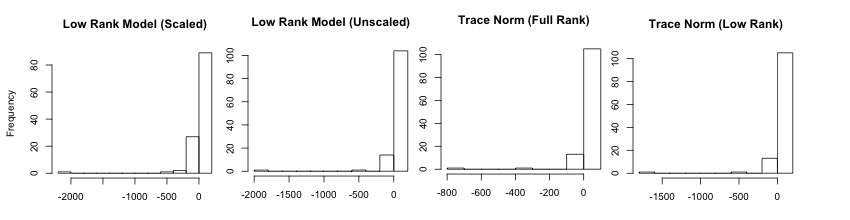
\includegraphics[width = 1.2\textwidth]{PercentGain_GSS.png}
\end{figure}

\begin{figure}[H]
\caption*{Column-wise lowest losses}
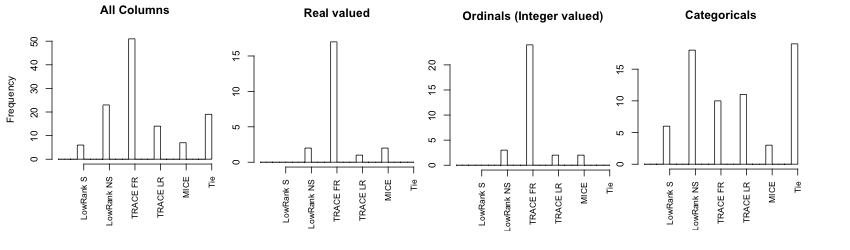
\includegraphics[width = 1.2\textwidth]{ColumnSelect_GSS.png}
\end{figure}


\newpage

\section*{Detailed Results -- Simulation data}

The results from the simulation are very similar to the GSS subsample:
\begin{itemize}
\item[1] Overall the Trace (Full Rank) had the lowest loss, about 25\% less than a single imputation using MICE. All the LowRankModels techniques did outperform MICE in terms of the total loss.
\item[2] If we look at the column-wise losses -- in general LowRankModels had lower total column loss for most columns (65\% for Trace (Full Rank)) and most of these columns had 30-50\% lower loss than MICE.
\item[3] However again for a few columns MICE had \textit{much} lower losses -- for one column it did 500\% better. 
\item[4] If we look at the type of column, we note that Trace (Full Rank) frequently has the lowest loss values for categorical columns and Low Rank (Scaled) for other columns.
\end{itemize}


% latex table generated in R 3.2.1 by xtable 1.7-4 package
% Thu Sep  3 13:43:57 2015
\begin{table}[H]
\caption*{Comparison of Imputation Techniques (scaled simulation data)} 
\centering
\begin{tabular}{|c|c|c|c|c|c|}
  \hline
 & LowRank (S) & LowRank (NS) & Trace (FR) & Trace (LR) & MICE \\ 
  \hline
Scaled Loss/($10^3$) & 1.60 & 1.40 & 1.40 & 1.40 & 1.80 \\ 
  \% reduction (wrt MICE) & 9.30 \% & 24.60 \% & 25.10 \% & 22.70 \% & -- \\ 
  \% columns with lower loss & 78.30  \%& 65.20  \%& 65.20 \% & 69.60 \% & -- \\ 
   \hline
\end{tabular}
\end{table}


\begin{figure}[H]
\caption*{Percent reduction in loss on using LowRankModels vs MICE}
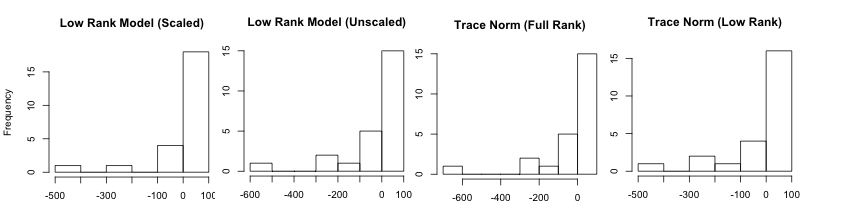
\includegraphics[width = 1.2\textwidth]{PercentGain_Simulated}
\end{figure}

\begin{figure}[H]
\caption*{Column-wise lowest losses}
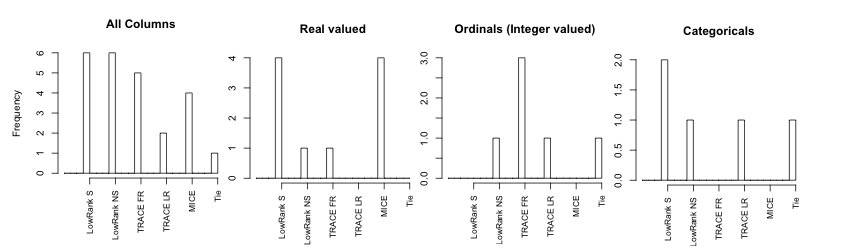
\includegraphics[width =1.2 \textwidth]{ColumnSelect_Simulated}
\end{figure}
























\end{document}